\externaldocument{Chapter5}
\externaldocument{Chapter4}
\externaldocument{Chapter3}

% Chapter 6

\chapter{Results}
\label{Chapter6}
\lhead{Chapter 6. \emph{Results}}

In this chapter, we will go over the results of the evaluation, which
is done as described in the previous chapter, "Evaluation
Plan"\ref{sec:evaluation_plan}. First comes the part where we discuss the
results we got when running the experiment using the framework. Here,
we describe how the experiment was orchestrated: what processes were
used, how the test file's code looked like. Then we'll take a look at
how the experiment was run, what information was given to the user
during runtime and how much time it took. Then, we will go over the
steps of the experiment done by hand, starting from connecting to the
interactive job started by the framework previously, then proceeding
with the experiment, describing certain details such as what commands
were needed to be given, or how much time the steps took. In the end,
we'll compare how the two different experimentation methods fare
against each other.
\section{Experiment using the framework}
First, we discuss the experiment orchestrated with the test
framework. The test written with the framework consists of one single
file, containing 1 method (the main) and 11 function calls. We can
look at the code on figure \ref{fig:experiment_code}.\\
The experiment itself can be divided into three main stages: the
preparation/configuration stage, the benchmark stage and the
post-processing stage.

\begin{figure}[htbp]
  \centering
    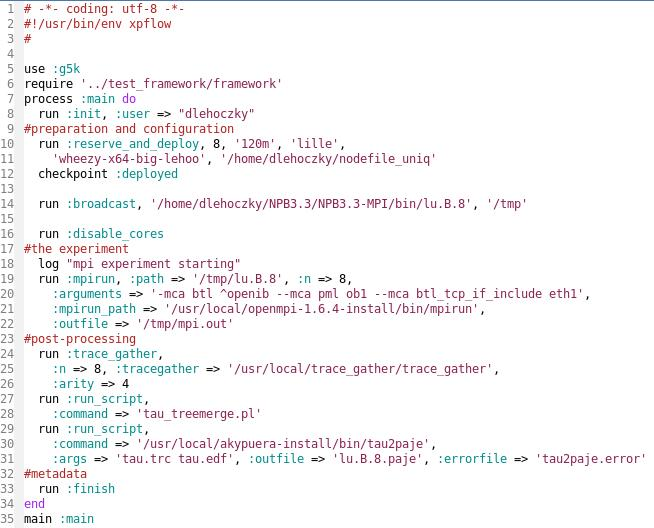
\includegraphics[scale=0.7]{./Figures/experiment_code.jpg}
    \rule{35em}{0.5pt}
  \caption[Experiment code]{The experiment, orchestrated with the test
    framework.}
  \label{fig:experiment_code}
\end{figure}

\subsection{Preparation}
\subsubsection{Experiment initialization}
In the beginning of every experiment, the \emph{init} method has to be
called in order to configure certain variables with default values and
also to make configuration steps regarding metadata collection
(e.g. record the date of the experiment, the exact time of starting,
etc.). Also, here is where the user can set his/her username to log in
to the nodes. If not set, the username will default to root.
\subsubsection{Reserve and deploy}
This is the part where the program starts a job by allocating 8 nodes
on the \emph{lille} site and deploying the image (given as a parameter
to the method) on them. We set the allocation time to 120 minutes (2
hours), which should give us plenty of time to execute the experiment
with both the framework and manually on the nodes.\\
As part of the process, a so-called 'nodefile' is created, which
contains the names of all the nodes that we allocated. Originally, the
environment variable \emph{\$OAR\_FILE\_NODES} is set on the frontend
when logged in to an active job, with the value of the path to a file
containing the node names, each as many times as many cores they
have. During the experiment, we create a nodefile that only contains
each node once, so it can be used as a machinefile for certain
commands later. We specify a custom path to the nodefile with an
argument. If that argument is not set, our nodefile would be created
in the home folder anyway.
\subsubsection{Broadcasting the runnable}
The benchmark needs to be copied to every node to the path where the
execution will take place - otherwise MPI wouldn't be able to start
its processes on every node. The parameters here are pretty
straightforward - we give the method the path to the compiled
benchmark and the path to copy it to. The nodefile is not needed to be
given, since it's already been created and stored by the library
before.
\subsubsection{Disabling cores}
This is the method call that is responsible for disabling all but one
core on every node that takes part in the execution. We talked about
why this is necessary earlier, see \ref{sec:multiple_cores}. No
parameters are needed to be given here.
\subsection{Running the benchmark}
After all the configuration steps have been successfully done, it's
time for actually running the benchmark. As parameters, we first give
the \emph{mpirun} method call the path to the runnable (meaning, of
course, the path that we broadcasted the runnable to before, not its
original path) and the number of nodes, which, in our case, is 8. We
also specify the MPI runnable with its full path: this is to avoid
confusion about which version of MPI is actually running on the nodes,
ensuring that it's the version we deployed on the image (OpenMPI
1.6.4). If not given, it would be defaulted to simply 'mpirun'. We
specify the file to put the output of the benchmark to as well.\\
We can put any extra arguments that we want to give to mpirun in the
"arguments" parameter. In this case, we use this parameter to specify
that our benchmark must not use Infiniband. This is needed because
SMPI is unable to simulate Infiniband connection, thus, a trace
acquired using it would show significantly better performance than the
simulated version.
\subsection{Post-processing}
\subsubsection{Gathering the traces}
As we mentioned before, in \ref{sec:experiment_process}, since we
compiled our benchmark with TAU, every MPI process produces
one trace (.trc) and one event (.evt) file. These traces are scattered
across the nodes. To gather them to one node, we use
the \emph{trace\_gather} MPI program. The method call with the same
name takes as parameter the number of nodes, the path to
the trace\_gather executable (the MPI executable is remembered
from the \emph{mpirun} call) and the arity parameter
(see \ref{sec:trace_gather}).
\subsubsection{Merging the traces}
For running \emph{tau\_treemerge.pl}, we use the \emph{run\_script}
method of the framework, which is a generic method that executes the
command given as parameter on the head node. No other arguments are
needed in this case. Although we could specify files to put the output
and the error messages to, we don't really need that in this simple
case. The directory to merge the traces in defaults to "/tmp", so that
is not needed either. As we mentioned before, this script doesn't only
merge our traces, it also attempts at accounting for any clock skew.
\subsubsection{Converting the traces}
As mentioned before, we use Akypuera's\cite{s13} \emph{tau2paje}
script to convert our traces to Pajé-visualizable format. For this, we
use the \emph{run\_script} method again, giving it the trace and event
files as arguments, as well as files to put the output and the error
messages to. Tau2paje generates error messages because of
synchronization problems (clock skew). As we described before
(see \ref{sec:clock_synch}), clock skew problems are really hard to
overcome. Although the merging script before tried to take care of the
problem, it can't eliminate it completely, but it does a well enough
job so this problem doesn't interfere with the conversion results in
any noticeable way.\\
After the conversion is done, the visualizable trace file called
\emph{lu.B.8.paje} is available on the /tmp folder of the head
node. We can now copy it to our local machine and visualize the
result. (The results will be discussed below, after discussing the
manual experiment.)
\subsection{Metadata}
In the end, we get some amount of metadata generated by the
experiment, summarizing some of its most important specifics, as it
can be seen on figure ref{}.\\
\#screenshot of the metadata\\
\section{Experiment by hand}
Now, let's take a look at how the manual experiment went. As mentioned
before, the two experiments consist of the same exact steps. As
before, we divide the experiment into three main sections:
preparation stage, benchmark stage and post-processing stage.
\subsection{Preparation}
Below is a table summarizing the results for the preparation and
configuration stage. The whole preparation stage took place on the
frontend of the site "lille", with the user "dlehoczky".
\renewcommand{\arraystretch}{1.5}
\begin{center}
\begin{spacing}{1}
\begin{tabular}{| p{4cm} | p{8cm} | l |} \toprule
  \multicolumn{3}{ |c| }{\textbf{Preparation}} \\ \midrule
  \multicolumn{1}{ |c| }{\emph{Task}} & \multicolumn{1}{ |c|
  }{\emph{Command}} & \multicolumn{1}{ |c| }{\emph{Time
  (s)}}\\ \midrule
  Reserving nodes & Omitted - joined the existing job,
  using the already allocated nodes & \\
  Deployment & \texttt{\small kadeploy3 -f \$OAR\_FILE\_NODES -e
  wheezy-x64-big-lehoo} & \\
  Create a nodefile containing all the node names only once
  & \texttt{\small cat   \$OAR\_FILE\_NODES | uniq > \textasciitilde
  /nodefile\_uniq} & \\
  Broadcast of runnable & \texttt{\small taktuk -l root -f
  \textasciitilde /nodefile\_uniq broadcast put
  { \$NPB\_DIR/bin/lu.B.8 } { /tmp }} & \\
  Disabling cores & \texttt{\small taktuk -l root -f /home/dlehoczky/nodefile\_uniq
  broadcast exec [ 'for i in /sys/devices/system/cpu/ cpu[1-9]*/online;
    do echo 0 > "\${i}" ; done' ]} & \\
  \emph{Optional}: Check if the cores have been disabled accordingly
  & \texttt{\small taktuk -f \textasciitilde /nodefile\_uniq broadcast
  exec [ 'cat /proc/cpuinfo' ] | grep process | awk '{if(\$9>0)
  print \$1}' | uniq | awk -F".fr-" '{print \$1".fr"}'} & \\ \midrule
\end{tabular}
\end{spacing}
\end{center}

As a side note: when doing the core disabling with the framework, the
program repeats the disabling step until it confirms it to be
successful, with the step marked as "Optional" here. In the step where
we check if the cores are disabled, every node name is displayed that
has more than 1 core running. The disabling step needs to be repeated
until we don't see any node names when running that command. When
running the test, the disabling step was successful the first time,
thus there was no need to repeat that step.
\subsection{Running the benchmark}
Below is the table about the command that was given to run the
benchmark (which is exactly the same as it was for the framework), as
well as its runtime. The benchmark had to be run from the directory
the benchmark was broadcasted to (/tmp in our case), on the designated
head node (which was, in our case, \#{TODO: head node}, the same as it
was for the framework.

\begin{center}
\begin{spacing}{1}
\begin{tabular}{| p{4cm} | p{8cm} | l |} \toprule
  \multicolumn{3}{ |c| }{\textbf{Running the benchmark}} \\ \midrule
  \multicolumn{1}{ |c| }{\emph{Task}} & \multicolumn{1}{ |c|
  }{\emph{Command}} &   \multicolumn{1}{ |c| }{\emph{Time
  (s)}}\\ \midrule
  Running the benchmark
  & \texttt{\small{/usr/local/openmpi-1.6.4-install
  /bin/mpirun -mca
  btl \textasciicircum openib --mca pml ob1 -machinefile
  \textasciitilde /nodefile\_uniq -np 8 /tmp/lu.B.8 1>/tmp/mpi.out}} & \\ \midrule
\end{tabular}
\end{spacing}
\end{center}

\subsection{Post-processing}
After executing the benchmark, the produced traces are sitting on
their respective nodes. Below, we summarize how the post-processing of
the files went. This stage of the experiment, as it was for the
benchmark, was executed on the head node, from the /tmp directory.

\begin{center}
\begin{spacing}{1}
\begin{tabular}{| p{4cm} | p{8cm} | l |} \toprule
  \multicolumn{3}{ |c| }{\textbf{Post-processing}} \\ \midrule
  \multicolumn{1}{ |c| }{\emph{Task}} & \multicolumn{1}{ |c|
  }{\emph{Command}} & \multicolumn{1}{ |c| }{\emph{Time
  (s)}}\\ \midrule
  Gathering the traces & \texttt{\small/usr/local/bin/mpirun
  -machinefile \textasciitilde /nodefile\_uniq -np 8
  /usr/local/trace\_gather/trace\_gather -f 1 -a 4 -m \textasciitilde
  /nodefile\_uniq} & \\
  Merging the traces & \texttt{\small tau\_treemerge.pl} & \\
  Converting the trace to Pajé-compatible format & \texttt{\small
  /usr/local/akypuera-install/bin/tau2paje tau.trc tau.edf
  1>lu.B.8.paje 2>tau2paje.error} & \\ \midrule
\end{tabular}
\end{spacing}
\end{center}

As mentioned previously at the end of the experiment with the
framework: after the conversion process, the file \emph{lu.B.8.paje}
is available on the head node, in its /tmp folder. Now, we can use
scp, rcp or some other program to download it to our local machine
from the remote node.
\section{Comparison}
First, let's take a look at how much time the experiments took. Below
is a table summarizing the elapsed time for both experiments.

\definecolor{light-gray}{gray}{0.90}
\begin{center}
\begin{spacing}{1}
\begin{tabular}{| c | c | c |} \toprule
  \multicolumn{1}{ |c|
  }{\multirow{2}{*}{\Large \textbf{\emph{Stage}}}} & \multicolumn{2}{
  |c| }{\textbf{\emph{Time (s)}}} \\ \cmidrule{2-3}
  & \multicolumn{1}{ |c| }{\emph{Experiment
  with the framework}} & \multicolumn{1}{ |c| }{\emph{Manual
  experiment}}\\ \midrule
  Preparation & - & - \\
  Running the benchmark & - & - \\
  Post-processing & - & - \\ \midrule
\end{tabular}
\end{spacing}
\end{center}

Now, let's take a look at the generated traces. Below are the results
for both experiments, visualized with Vite, a Pajé visualization tool.
\#TODO: visualizations here; below: compare them
advantages of the framework (obvious one: no user intervention
required during the process)
